\subsection{线性映射的指标}

设 L 是一个域 \(^{1}\) ，设 U 和 V 是两个向量空间 \(^{2}\) （在 L 上的）且 \(f: U \to V\) 是一个 L-线性映射；若 f 的核 N 与余核 C 具有有限维数，则称 f 具有有限指标，并且整数

\[
\chi (f) = [ \mathrm{C}: \mathrm{L} ] - [ \mathrm{N}: \mathrm{L} ]
\]

称为 \(f\) 的指标。

每个线性映射 \(f: \mathrm{U} \to \mathrm{V}\) 都具有指标，等于 \([\mathrm{V}: \mathrm{L}] - [\mathrm{U}: \mathrm{L}]\) 。设 \(\mathbf{N}\) 为核， \(\mathbf{I}\) 为像， \(\mathbf{C}\) 为 \(f\) 的余核。我们有 \(\mathbf{C} = \mathbf{V} / \mathbf{I}\) 且 \(\mathbf{I}\) 同构于 \(\mathbf{U} / \mathbf{N}\) ；因此我们有 \([\mathrm{U}: \mathrm{L}] = [\mathrm{N}: \mathrm{L}] + [\mathrm{I}: \mathrm{L}]\) 且 \([\mathrm{V}: \mathrm{L}] = [\mathrm{C}: \mathrm{L}] + [\mathrm{I}: \mathrm{L}]\) ，由此即得结果。

引理 2. --- 设 \(f: \mathbf{U} \to \mathbf{V}\) 和 \(g: \mathbf{V} \to \mathbf{W}\) 是两个 L-线性映射。如果 \(f\) 和 \(g\) 每一个都有指标，那么 \(g \circ f\) 亦然，并且我们有

\[
\chi (g \circ f) = \chi (f) + \chi (g).
\]

令 \(h = g \circ f\) ，并用 \(\mathbf{N}, \mathbf{N}'\) , \(\mathbf{N}''\) 分别记 \(f, g, h\) 的核，用 \(\mathbf{C}, \mathbf{C}'\) , \(\mathbf{C}''\) 记它们的余核。我们有 \(\mathbf{N} \subset \mathbf{N}'' \subset \mathbf{U}\) 且 \(f(\mathbf{N}^{\prime\prime}) = f(\mathbf{U}) \cap \mathbf{N}'\) ；因此存在一个线性映射 \(\bar{f}: \mathbf{N}^{\prime\prime} \to \mathbf{N}'\) ，它与 \(f\) 在 \(\mathbf{N}''\) 上一致且核为 \(\mathbf{N}\) 。典范映射 \(\pi\) （\(\mathbf{V}\) 映到 \(\mathbf{C} = \mathbf{V}/f(\mathbf{U})\) 上的）诱导出一个映射 \(\pi'\) （\(\mathbf{N}'\) 到 \(\mathbf{C}\) 中的），其核为 \(f(\mathbf{U}) \cap \mathbf{N}' = \bar{f}(\mathbf{N}^{\prime\prime})\) 。通过取商， \(g\) 定义了一个映射 \(\bar{g}\) （\(\mathbf{C} = \mathbf{V}/f(\mathbf{U})\) 到 \(\mathbf{C}'' = \mathbf{W}/g(f(\mathbf{U}))\) 中的），其核显然为 \((\mathbf{N}' + f(\mathbf{U}))/f(\mathbf{U}) = \pi'(\mathbf{N}')\) 。最后，典范映射 \(\rho\) （\(\mathbf{C}'' = \mathbf{W}/g(f(\mathbf{U}))\) 映到 \(\mathbf{C}' = \mathbf{W}/g(\mathbf{V})\) 上的）的核为 \(g(\mathbf{V})/g(f(\mathbf{U})) = \bar{g}(\mathbf{C})\) 。综上所述，我们已建立了序列的正合性

\[
0 \to \mathrm{N} \stackrel {i} {\to} \mathrm{N} ^ {\prime \prime} \stackrel {\bar {f}} {\to} \mathrm{N} ^ {\prime} \stackrel {\pi^ {\prime}} {\to} \mathrm{C} \stackrel {\bar {g}} {\to} \mathrm{C} ^ {\prime \prime} \stackrel {\rho} {\to} \mathrm{C} ^ {\prime} \to 0
\]

（其中 \(i\) 是 \(\mathbf{N}\) 到 \(\mathbf{N}''\) 中的典范单射）。

\pandocbounded{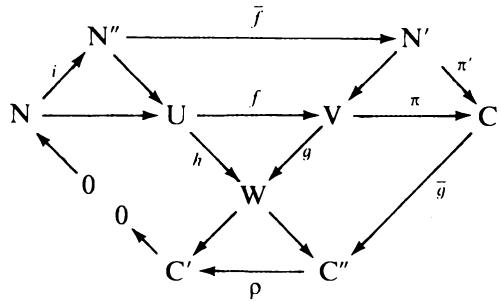
\includegraphics[keepaspectratio]{images/part002_9769358f.jpg}}\\
图 1

根据假设，N、N'、C 和 C' 都是有限维的；因此 N'' 和 C'' 也是如此。由推论 2（II，第 295 页）我们于是有

\[
[ \mathrm{N}: \mathrm{L} ] - [ \mathrm{N} ^ {\prime \prime}: \mathrm{L} ] + [ \mathrm{N} ^ {\prime}: \mathrm{L} ] - [ \mathrm{C}: \mathrm{L} ] + [ \mathrm{C} ^ {\prime \prime}: \mathrm{L} ] - [ \mathrm{C} ^ {\prime}: \mathrm{L} ] = 0
\]

由此 \(\chi(h) = \chi(f) + \chi(g)\) 。

